\documentclass[12pt, twoside]{article}
\usepackage[letterpaper, margin=1in, headsep=0.5in]{geometry}
\usepackage[english]{babel}
\usepackage[utf8]{inputenc}
\usepackage{amsmath}
\usepackage{amsfonts}
\usepackage{amssymb}
\usepackage{tikz}
%\usetikzlibrary{quotes, angles}

\usepackage{graphicx}
\usepackage{enumitem}
\usepackage{multicol}

\usepackage{fancyhdr}
\pagestyle{fancy}
\fancyhf{}
\renewcommand{\headrulewidth}{0pt} % disable the underline of the header

\fancyhead[RE]{\thepage}
\fancyhead[RO]{\thepage \\ Name: \hspace{3cm}}
\fancyhead[L]{BECA / Dr. Huson / 10th Grade Geometry\\* 12 December 2018}

\begin{document}
\subsubsection*{Do Now: Triangle congruence proofs}
 \begin{enumerate}

\item Given $\triangle ABP$ and $\triangle JKP$ with $\angle B \cong \angle K$. $P$ bisects $\overline{AJ}$. Prove $\triangle ABP \cong \triangle JKP$.\\[0.5cm]
  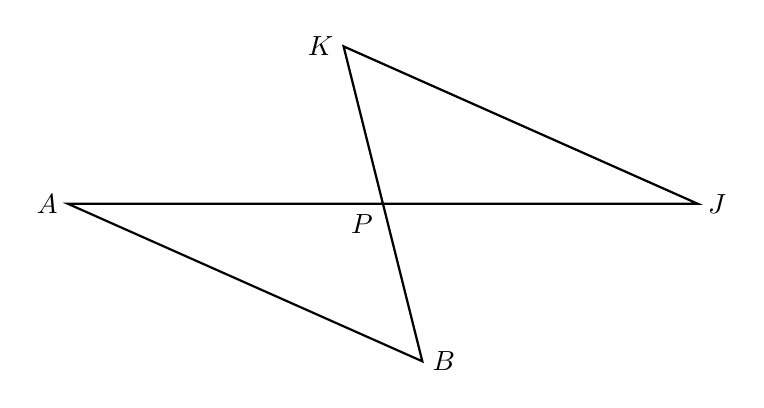
\begin{tikzpicture}
      \draw [thick]
        (0.5,-2)node[right]{$B$}--
        (-0.5,2)node[left]{$K$}--
        (4,0)node[right]{$J$}--
        (0,0)node[below left]{$P$}--
        (-4,0)node[left]{$A$}--cycle;
    \end{tikzpicture}

  \begin{multicols}{2}
    \underline{Statement} \\
    \underline{Reason}
  \end{multicols}
  \begin{multicols}{2}
    \raggedcolumns
    \begin{enumerate}[label={\arabic*)}]
      \item $\triangle ABP$, $\triangle JKP$ \vspace{0.3cm}
      \item \rule{4cm}{0.15mm} \vspace{0.3cm}
      \item \rule{4cm}{0.15mm} \vspace{0.3cm}
      \item $\angle APB \cong \angle JPK$  \vspace{0.3cm}
      \item \rule{4cm}{0.15mm} \vspace{0.3cm}
      \item $\triangle ABP \cong \triangle JKP$ \vspace{0.3cm}
    \end{enumerate}
    \begin{enumerate}[label={\arabic*)}]
      \item Given \vspace{0.3cm}
      \item Given \vspace{0.3cm}
      \item Given \vspace{0.3cm}
      \item \rule{4cm}{0.15mm} \vspace{0.3cm}
      \item Definition of a bisector \vspace{0.3cm}
      \item \rule{4cm}{0.15mm} \vspace{0.3cm}
    \end{enumerate}
  \end{multicols}

  \item $M(5,5)$ is the midpoint of $AB$. Given $A(2,3)$, find the other endpoint, $B$. \vspace{2cm}

  \item The line $l$ has the equation $y=\frac{1}{2} x-3$.
    \begin{enumerate}
      \item What is the slope of the line $k$, given $k \parallel l$?
      \vspace{1cm}
      \item What is the slope of the line $m$, given $m \perp l$?
      \vspace{1cm}
    \end{enumerate}

    \item A translation maps $A(5,2) \rightarrow A'(-2,3)$. What is the image of $B(-1,5)$ under the same translation?  \vspace{0.5cm}


\newpage
\subsubsection*{Early finishers}

\item Using  a  compass  and  straightedge,  construct  the  median  to  side $\overline{AB}$ in $\triangle ABC$ below.\\ (Leave all construction marks.)
  \vspace{1cm}
\begin{center}
\begin{tikzpicture}
  \draw [<->, thick]
    (0,0) node[left]{$A$}--
    (10,-2) node[right]{$B$}--
    (4,-5) node[below]{$C$}
    --cycle;
\end{tikzpicture}
\end{center}

  \vspace{2cm}

\item With a compass and straightedge, construct a square inscribed in circle $Q$. (Leave all construction marks.)
  \vspace{1cm}
  \begin{center}
  \begin{tikzpicture}
  \draw [thick] (0,0) circle [radius=4cm];
  \draw [fill] (0,0) circle [radius=0.05] node[below]{$Q$};
  \end{tikzpicture}
  \end{center}

\end{enumerate}
\end{document}
